\documentclass[UTF8]{ctexart}
\usepackage{amsmath}
\usepackage{amssymb}
\usepackage{bm}
\usepackage{booktabs}
\usepackage{breqn}
\usepackage{color}
\usepackage{enumitem}
\usepackage{float}
\usepackage[backend=bibtex,bibstyle=gb7714-2015,citestyle=gb7714-2015]{biblatex}
\setlength{\bibitemsep}{3bp}
\renewcommand*{\bibfont}{\zihao{5}\linespread{1.27}\selectfont}
\addbibresource{ref.bib}
\usepackage{graphicx}
\usepackage{hyperref}
\usepackage{indentfirst}
\usepackage{multicol}
\usepackage{ntheorem}
\usepackage{subfigure}
\usepackage{txfonts}
\usepackage{algorithm}
\usepackage{algorithmic}
\setlength{\parindent}{2em}
\usepackage{IEEEtrantools}
\usepackage{geometry}
\usepackage{listings}
\usepackage{lastpage}
\usepackage{tikz}
\usepackage{chngpage}
%\lstset{
%	commentstyle=\color{red!50!green!50!blue!50},%代码块背景色为浅灰色
%	rulesepcolor= \color{gray}, %代码块边框颜色
%	breaklines=true,  %代码过长则换行
%	numbers=left, %行号在左侧显示
%	numberstyle= \small,%行号字体
%	keywordstyle= \color{blue},%关键字颜色
%	frame=shadowbox,%用方框框住代码块
%	basicstyle=\ttfamily
%}
\definecolor{dkgreen}{rgb}{0,0.6,0}
\definecolor{mauve}{rgb}{0.9,0.1,0.4}
\definecolor{ash}{rgb}{0.8,0.8,0.8}
\lstset{ 
	language=Octave,                % the language of the code
	basicstyle=\ttfamily,           % the size of the fonts that are used for the code
	numbers=left,                   % where to put the line-numbers
	numberstyle=\small\color{gray},  % the style that is used for the line-numbers
	stepnumber=1,                   % the step between two line-numbers. If it's 1, each line
	% will be numbered
	numbersep=5pt,                  % how far the line-numbers are from the code
	backgroundcolor=\color{ash},      % choose the background color. You must add \usepackage{color}
	rulesepcolor= \color{gray}, %代码块边框颜色
	showspaces=false,               % show spaces adding particular underscores
	showstringspaces=false,         % underline spaces within strings
	showtabs=false,                 % show tabs within strings adding particular underscores
	frame=single,                   % adds a frame around the code
	rulecolor=\color{black},        % if not set, the frame-color may be changed on line-breaks within not-black text (e.g. commens (green here))
	tabsize=2,                      % sets default tabsize to 2 spaces
	captionpos=b,                   % sets the caption-position to bottom
	breaklines=true,                % sets automatic line breaking
	breakatwhitespace=false,        % sets if automatic breaks should only happen at whitespace
	title=\lstname,                   % show the filename of files included with \lstinputlisting;
	% also try caption instead of title
	frame=shadowbox,%用方框框住代码块
	keywordstyle=\color{blue},          % keyword style
	commentstyle=\color{dkgreen},       % comment style
	stringstyle=\color{mauve},         % string literal style
	escapeinside={\%*}{*)},            % if you want to add LaTeX within your code
	morekeywords={*,...}               % if you want to add more keywords to the set
}
\graphicspath{{figs/}}
\floatname{algorithm}{算法}  
\renewcommand{\algorithmicrequire}{\textbf{输入:}}  
\renewcommand{\algorithmicensure}{\textbf{输出:}} 
\author{
	吴熙楠}
\title{
	\heiti{受激布里渊散射陀螺仪}
}

\hypersetup{
	colorlinks=true,
	linkcolor=black
}


\begin{document}
	\maketitle
	\newtheorem{definition}{定义}[subsection]
	\newtheorem{function}{公式}[subsection]
	\newtheorem{summary}{小结}[subsection]
	\newtheorem{deduction}{推论}[subsection]
	\newtheorem{property}{性质}[subsection]
	\newtheorem{theo}{定理}[subsection]
	\newtheorem{step}{步骤}[subsection]
	\newtheorem{remark}{注记}[subsection]
	\newtheorem{proof}{证明}[subsection]
	\newenvironment{Theorem}[1][]{\par\noindent\textbf{定理}(#1)\quad}{\par}
	\newcommand{\rbra}[1]{\left( #1 \right)}
	\newcommand{\sbra}[1]{\left[ #1 \right]}
	\newcommand{\cbra}[1]{\left\{ #1 \right\}}
	\newcommand{\pbra}[1]{\left< #1 \right>}
	\newcommand{\abs}[1]{\left| #1 \right|}
	\newcommand{\fs}[2]{\displaystyle\frac{#1}{#2}}
	
	\newenvironment{myproof}{{\color{blue}证:}}
	
	\newenvironment{partlist}[1][]
	{\begin{enumerate}[itemsep=0pt, label=(\arabic*), wide, labelindent=\parindent, listparindent=\parindent, #1]}
		{\end{enumerate}}
	
	\renewcommand{\contentsname}{目录} %将content转为目录
	\tableofcontents
	\newpage
	\renewcommand{\abstractname}{\large 摘要\\}
	\begin{abstract}
		布里渊散射光纤陀螺仪是新一代小型化高精度光纤陀螺仪,随着光纤通讯和光纤传感技术的发展,布里渊光纤环形激光器迅速发展并得到了广泛应用。当光纤环中光强达到一定程度就会出现布里渊散射,散射光频率受到$Sagnac$效应影响,我们可以检测散射光频率得到光纤环的旋转速度,由于可以直接给出频率输出,被认为是具有吸引力的新一代陀螺。
		
		\textbf{关键词:布里渊散射,$Sagnac$效应,光纤环}
	\end{abstract}
\section{布里渊光纤陀螺研究历史}
1964年,R. Y. Chiao等人首次观察到了受激布里渊散射现象。20世纪六七十年代,激光器技术快速发展,固体激光器、气体激光器和半导体激光器相继问世,这些都为布里渊光纤环形激光器的发明奠定了基础。


第一个连续波泵浦的布里渊光纤环形激光器由Hill等人在1976年制作出来。该激光器采用波长$0.5145 \mu m $的氩离子激光器作为泵浦,采用长度$9.5 m$、纤芯直径$2.4 \mu m$ 、数值孔径0.1的单模光纤,光纤损耗小于$100 dB/km$,环形腔由光纤和分束器组成。实验观测到了一个带宽为$20 MHz$、布里渊频移为$34 GHz$的单峰,并没有观测到预想中频率间隔为$10 MHz$的多个纵模。实验还测得$Stokes$光的抽运阈值小于$100 mW$,只有30\%的光功率通过分束器耦合进环形腔。Hill等人制作的布里渊环形腔的主要优点是具有连续的高转化效率,他们还将谐振腔截断证明了反馈可以降低抽运阈值,并提出了用低损耗长光纤制作谐振腔可以进一步降低抽运阈值的假设。


Smith等人还提出了同腔布里渊光纤环形激光器,方向相反的两束泵浦光产生的两束$Stokes$光在同一谐振腔内运转并通过方向耦合器输出,它们的拍频通过一个光电二极管进行检测并由频谱仪进行分析,同腔布里渊光纤环形激光器主要应用于布里渊光纤陀螺。


布里渊光纤陀螺由 Thomas在 1980 年提出,但由于当时实验条件的限制,没有观测到两束 Stokes 光产生的拍频。20 世纪 80 年代末 90 年代初,R. K. Kadiwar、F. Zarinetchi、Michael Raab、S. Huang、K. Hotate等人分别提出了布里渊光纤陀螺方案,这些方案验证了布里渊光纤环形激光器用于惯性测量的可行性,在实验中发现了一些问题并提出了相应的解决措施。图 1\cite{Luo2013BrillouinRamanCO} 为 F. Zarinetchi 等人提出的布里渊光纤陀螺方案,用波长 $1.15 \mu m$ 的单纵模 $He-Ne$ 激光器作泵浦源,泵浦光由分束器分为 P1 和 P2两束,使用声光调制器和耦合器使两束光以不同的频率(相差 12 个纵模间隔,$92.4 MHz$)沿相反的方向耦合进光纤谐振腔,环形腔由总长 25 m 的单模光纤构成,P1、P2 产生的 $Stokes$ 光 B1、B2通过分束器 BS1 同时输出。实验结果表明,当布里渊光纤陀螺的旋转角速度以正弦函数变化时,可以观察到稳定的拍频信号,拍频信号的波形为中心频率$ 92.4 MHz$ 的正弦函数。
\begin{figure}[htb]
	\begin{center}
		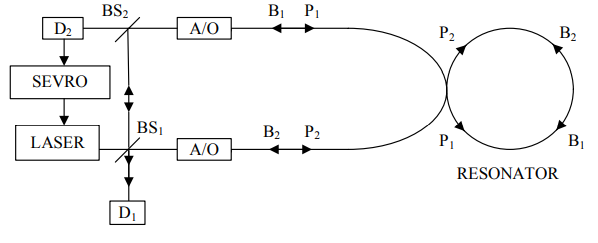
\includegraphics[width=0.7\textwidth]{1.png}
		\caption{F. Zarinetchi等人提出的布里渊光纤陀螺结构示意图}
	\end{center}
\end{figure}
\section{布里渊光纤陀螺理论}
$BFOG$由高功率窄谱激光光源、光纤谐振器和信号处理单元组成。激光器的泵浦光通过光纤耦合器进入光纤谐振腔,光功率的增加导致第一阶$Stokes$光波B1和B2的传播方向与泵浦光P1和P2相反。无论是$BFOG$中的$Sagnac$效应,还是谐振频率的变化,都会导致B1和B2的谐振频率发生差异,从而产生干扰,干扰信号由检测电路进行处理。当泵浦光功率超过布里渊散射阈值功率时,泵浦光功率的增加将导致第一阶$Stokes$光功率的增加,并刺激产生二阶和高阶$Stokes$光波,如图\cite{Lihui2015MathematicalMO}:
\begin{figure}[htb]
	\begin{center}
		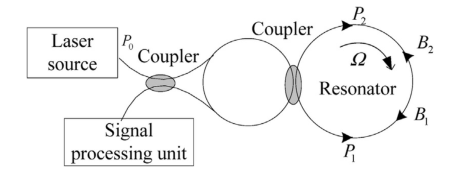
\includegraphics[width=0.7\textwidth]{2.png}
		\caption{BFOG的基本结构}
	\end{center}
\end{figure}


我们给出了光纤谐振腔激发一阶$Stokes$光波的布里渊散射阈值强度$I_{c,th}$:
\begin{equation}
	\begin{aligned}
		I_{c,th}&=\dfrac{2A_{eff}}{g_{B}L}(\gamma +\alpha L)\\
		R&=\sqrt{1-\kappa}\sqrt{1-\gamma}e^{-\alpha L/2}
	\end{aligned}
\end{equation}


其中$R$为振幅透射系数,$g_{B}$为布里渊增益系数,$A_{eff}$为光纤的有效截面积,$\gamma$为光纤耦合器损耗系数,$\alpha$为光纤环的传输损耗系数,$L$为谐振腔长度,$\kappa$为耦合器的强度耦合系数。


激光激发一阶$Stokes$光波的阈值强度为:
\begin{equation}
	\begin{aligned}
		I_{p,th}=\dfrac{2A_{eff}}{g_{B}L}\dfrac{(\gamma+\alpha L)^{2}}{1-\gamma}
	\end{aligned}
\end{equation}


我们给出了泵浦和$Stokes$光波沿光纤谐振腔长度分布的微分方程:
\begin{equation}
	\begin{aligned}
		\dfrac{dI_{s}(z)}{dz}&=-g_{B}I_{p}I_{s}+\alpha I_{s}\\
		\dfrac{dI_{p}(z)}{dz}&=-g_{B}I_{p}I_{s}-\alpha I_{p}\\
		I_{p}(z)&=I_{P}(0)e^{-\alpha z}
	\end{aligned}
\end{equation}


我们可以由此解得斯托克斯光强为:\begin{equation}
	\begin{aligned}
		I_{s}(0)&=I_{s}(L)e^{g_{B}I_{p}(0)L_{eff}-\alpha L}\\
		L_{eff}&=\dfrac{1}{\alpha}(1-e^{-\alpha L})
	\end{aligned}
\end{equation}


因此,激发一阶$Stokes$光波所需的阈值功率为:
\begin{equation}
	\begin{aligned}
		P_{th}=G\dfrac{K_{B}A_{eff}}{g_{B}L_{eff}}=G\dfrac{K_{B}A_{eff}\alpha}{g_{B}(1-e^{-\alpha L})}
	\end{aligned}
\end{equation}


其中$K_{B}$是由偏振度决定的偏振因子,$L_{eff}$是光纤的有效长度,$G$是总布里渊增益系数。


结果表明,阈值功率受光纤长度和光纤损耗的影响,因此,具有较低损耗的较长的光纤将产生较低的阈值功率。


光纤谐振器的原理图如下图\cite{Nelson2019ReducingNI}所示:
\begin{figure}[H]
	\begin{center}
		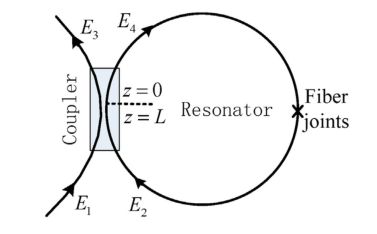
\includegraphics[width=0.6\textwidth]{3.png}
		\caption{光纤谐振器原理图}
	\end{center}
\end{figure}


配光场分量关系如下:
\begin{equation}
	\begin{aligned}
		&|E_{3}|^{2}+|E_{4}|^{2}=(1-\gamma)(|E_{1}|^{2}+|E_{2}|^{2})\\
		&E_{2}=E_{4}(1-\alpha_{0})e^{-\alpha L+i\beta L}\\
		&E_{3}=E_{1}\dfrac{\sqrt{1-\gamma}}{\sqrt{1-\kappa}}(1-\dfrac{\kappa}{1-\sqrt{(1-\kappa)(1-\alpha_{0})(1-\gamma)e^{-2\alpha L}}e^{i\beta L}})\\
		&E_{4}=E_{1}\dfrac{i\sqrt{1-\gamma}\sqrt{\kappa}}{\sqrt{1-\kappa}-\sqrt{(1-\kappa)(1-\alpha_{0})(1-\gamma)e^{-2\alpha L}}e^{i\beta L}}
	\end{aligned}
\end{equation}


其中$\beta L$为光波在光纤环路传播的相位,$\alpha_{0}$为光纤接头损耗。


在最佳共振下,谐振器耦合器出口能量为0,则:\begin{equation}
	\begin{aligned}
		1-\dfrac{\kappa}{1-\sqrt{(1-\kappa)(1-\alpha_{0})(1-\gamma)e^{-2\alpha L}}e^{i\beta L}}=0
	\end{aligned}
\end{equation}


令$M=(1-\kappa)(1-\alpha_{0})(1-\gamma)e^{-2\alpha L}$,则:
\begin{equation}
	\begin{aligned}
		&1-\kappa-\sqrt{M}cos(\beta L)=i\sqrt{M}sin(\beta L)\\
		&\beta L=q\cdot 2\pi\\
		&\kappa=1-(1-\gamma)(1-\alpha_{0})e^{-2\alpha L}
	\end{aligned}
\end{equation}


由上式我们可以求得配光场分量在产生最佳谐振时之间的关系。


$SBS$光纤$RLG$系统一般由三部分组成:输入/输出子系统、反馈子系统和$SBS$光纤环形谐振器,如图所示\cite{Luo2013BrillouinRamanCO}:
\begin{figure}[H]
	\begin{center}
		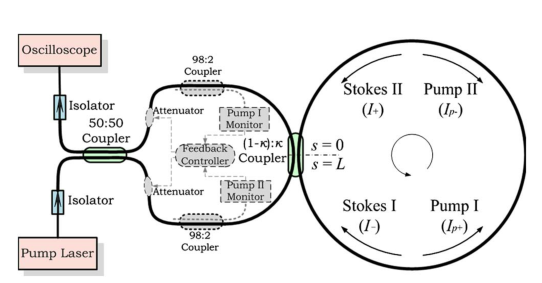
\includegraphics[width=0.6\textwidth]{4.png}
		\caption{SBS光纤RLG的实验装置}
	\end{center}
\end{figure}


我们可以通过扰动方程计算出强度和相位关系:\begin{equation}
	\begin{aligned}
		\dfrac{\dot{I_{\pm}}}{I_{\pm}}&=-\dfrac{P_{m}}{u}\alpha_{L}+\dfrac{2\omega_{m}}{u}\dfrac{\kappa_{sp}\gamma^{2}\chi_{B}I_{p\mp}}{(\Omega-\omega_{p\mp}+\omega_{\pm})^{2}+\gamma^{2}}-\dfrac{2\omega_{m}}{u}[2\kappa_{sp}\chi_{T}(I_{p+}+I_{p-})+\kappa_{ss}\chi_{T}(2I_{\mp}+I_{\pm})]\\
		\dot{\phi_{\pm}}&=\dfrac{\omega_{m}}{u}\dfrac{\kappa_{sp}\gamma(\Omega-\omega_{p\mp}+\omega_{\pm})\chi_{B}I_{p\mp}}{(\Omega-\omega_{p\mp}+\omega_{\pm})^{2}+\gamma^{2}}+\dfrac{\omega_{m}}{u}[2\kappa_{sp}\chi_{K}(I_{p+}+I_{p-})+\kappa_{ss}\chi_{K}(2I_{\mp}+I_{\pm})]\\
		\kappa_{sp}&=\dfrac{1}{4}\iint\epsilon_{0}(\hat{E_{m}^{\star}}\cdot\hat{E_{m}})^{2}d\sigma\\
		\kappa_{ss}&=\dfrac{1}{4}\iint\epsilon_{0}(\hat{E_{m}^{\star}}\cdot\hat{E_{m}})(\hat{E_{p}^{\star}}\cdot\hat{E_{p}})d\sigma
	\end{aligned}
\end{equation}


同理我们可以计算出这些反向传播的斯托克斯波的拍频为:\begin{equation}
	\begin{aligned}
		\omega_{B}=&\omega_{m}\dfrac{\kappa_{ss}}{u}\chi_{K}\Delta I+\omega_{m}\gamma\dfrac{\kappa_{sp}}{u}\dfrac{[(\Omega-\omega_{p+}+\omega_{-})(\Omega-\omega_{p-}+\omega_{+})-\gamma^{2}](\Delta \omega_{p}+\Delta\omega)}{[(\Omega-\omega_{p+}+\omega_{-})^{2}+\gamma^{2}][(\Omega-\omega_{p-}+\omega_{+})^{2}+\gamma^{2}]}\chi_{B} I_{p}\\&+\omega_{m}\gamma\dfrac{\kappa_{sp}}{u}\dfrac{[(\Omega-\omega_{p+}+\omega_{-})(\Omega-\omega_{p-}+\omega_{+})-\gamma^{2}](\Omega-\omega_{p}+\omega)}{[(\Omega-\omega_{p+}+\omega_{-})^{2}+\gamma^{2}][(\Omega-\omega_{p-}+\omega_{+})^{2}+\gamma^{2}]}\chi_{B}\Delta I_{p}
	\end{aligned}
\end{equation}


其中,$\chi_{K},\chi_{T},\chi_{B}$分别为Kerr系数、TPA系数和SBS系数。


我们即可以通过观察到的拍频以及已知参数计算出陀螺转速。
\section{布里渊光纤陀螺研究前景}
布里渊光纤陀螺目前存在的主要问题和解决方案有\cite{洪伟2010布里渊光纤环形激光器的发展与应用}:


(1)单频 SBS 激光的产生及稳定输出:系统的输出为拍频信号,这就要求布里渊激光器必须有稳定的单频输出。实现激光单纵模输出的方法很多,例如,采用短腔结构,即减小谐振腔的长度来增大相邻纵模的间隔,这样使工作介质的增益光谱范围内只存在一个纵模频率,从而使输出激光中只存在一个纵模。


(2)锁定现象:布里渊光纤陀螺旋转角速度小的时候没有拍频信号产生,目前对于这种现象没有完美的解决方案,但可以通过偏频法、推拉式相位调制法、光克尔效应法等方案来减小产生锁定的角速度范围。


(3)角速度方向的判断:拍频信号只能给出旋转角速度的大小,而不能给出旋转方向,因此如何判断角速度方向也是布里渊光纤陀螺必须考虑的问题。偏频法及推拉式相位调制法均可以很好地解决这一问题。


(4)偏振波动:布里渊光纤陀螺谐振腔中有两个互相垂直的本征偏振态。环境温度等因素的变化会使光纤中的双折射发生变化,从而使两个偏振本征态的传播常数发生变化,而这种变化对于两个沿相反方向传播$ Stokes $光来说不是完全一致的,因此,可能在陀螺输出中引入了频率差。现有的解决措施主要有 $90^{\circ}$偏振主轴偏置和采用单模光纤两种方案。


布里渊散射陀螺仪目前的应用状况:战略导弹系统和核潜艇导航应用,卫星定向和跟踪,战术武器制导与控制系统,应用于各种运载火箭,应用于陆地导航系统,天体观测望远镜的稳定与调向等。
\section{总结与展望}
布里渊光纤环形激光器因具有线宽窄、频率稳定、增益方向敏感等优点而被广泛研究,并在越来越多的领域得到应用。布里渊光纤陀螺的原理比干涉式光纤陀螺更先进,若能将现有的技术问题解决,布里渊光纤陀螺必将取代干涉式光纤陀螺,在未来的惯性导航系统中占据一席之地。
\printbibliography[heading = bibintoc]
\end{document}